\onehalfspacing
\section{Đề số 14}
\graphicspath{{./img/}}
\begin{bt} 
    \hfill
	\begin{enumerate}[a.]
		\item Cho biểu thức: $\mathrm{P}=\mathrm{x}-4 \mathrm{xy}+\mathrm{y}$. Tính giá trị của $\mathrm{P}$ với $|x|=1,5 ; \mathrm{y}=-0,75$
        \item Rút gọn biểu thức: $\mathrm{A}=\frac{2^{12} \cdot 3^5-4^6 \cdot 81}{\left(2^2 \cdot 3\right)^6+8^4 \cdot 3^5}$
	\end{enumerate}
	\loigiai{
        \begin{enumerate}
            \item Ta có: $|x|=1,5 \Rightarrow x=1,5$ hoặc $\mathrm{x}=-1,5$\\[4pt]
            +) Với $x=1,5$ và $y=-0,75$ thì\\[4pt]
            $\mathrm{P}=1,5-4.1,5(-0,75)-0,75=1,5(1+3)=6-0,75=5,25$\\[4pt]
            +) Với $x=-1,5$ và $y=-0,75$ thì\\[4pt]
            $\mathrm{P}=-1,5-4(-1,5) \cdot(-0,75)-0,75=-1,5(1+3)-0,75=-6,75$
            \item $\mathrm{A}=\frac{2^{12} \cdot 3^5-4^6 \cdot 81}{\left(2^2 \cdot 3\right)^6+8^4 \cdot 3^5}=\frac{2^{12} \cdot 3^5-2^{12} \cdot 3^4}{2^{12} \cdot 3^6-2^{12} \cdot 3^5}=\frac{2^{12} \cdot 3^4(3-1)}{2^{12} \cdot 3^5(3-1)}=\frac{1}{3}$
        \end{enumerate}
    } 
\end{bt}

\begin{bt}
	\hfill
	\begin{enumerate}[a.]
		\item Tìm $x, y, z$, biết:
        $$
        2 x=3 y ; 4 y=5 z \text { và } x+y+z=11
        $$
        \item Tìm $x$, biết: $|x+1|+|x+2|+|x+3|=4 x$
	\end{enumerate}
	\loigiai{
        \begin{enumerate}
            \item $2 x=3 y ; 4 y=5 z \Rightarrow \frac{x}{3}=\frac{y}{2} ; \frac{y}{5}=\frac{z}{4} \Rightarrow \frac{x}{15}=\frac{y}{10} ; \frac{y}{10}=\frac{z}{8} \\[5pt]
            \Rightarrow \frac{x}{15}=\frac{y}{10}=\frac{z}{8}=\frac{x+y+z}{15+10+8}=\frac{11}{33}=\frac{1}{3}\\[5pt] 
            \Rightarrow x=5 ; y=\frac{10}{3} ; z=\frac{8}{3}$
            \item $|x+1|+|x+2|+|x+3|=4 x$\\[5pt]
            Vì VT $\geq 0 \Rightarrow 4 x \geq 0$ hay $\mathrm{x} \geq 0$, do đó:\\[5pt]
            $|x+1|=x+1 ;|x+2|=x+2 ;|x+3|=x+3$\\[5pt]
            (1) $\Rightarrow x+1+x+2+x+3=4 x \quad \Rightarrow x=6$
        \end{enumerate}
    } 
\end{bt}

\begin{bt}
	Cho hàm số: $\mathrm{y}=\mathrm{f}(\mathrm{x})=-4 \mathrm{x}^3+\mathrm{x}$
	\begin{enumerate}[a.]
		\item Tính $f(0), f(-0,5)$
        \item Chứng minh: $f(-a)=-f(a)$.
	\end{enumerate}
	\loigiai{
        \begin{enumerate}
            \item $f(0)=0 \\[5pt]
            f(-0,5)=-4 \cdot\left(-\frac{1}{2}\right)^3-\frac{1}{2}=\frac{1}{2}-\frac{1}{2}=0 $
            \item $f(-a)=-4(-a)^3-a=-4 a^3-a \\[5pt]
            -f(a)=-\left[-4 a^3+a\right]=4 a^3-a \\[5pt]
            \Rightarrow f(-a)=-f(a)$
        \end{enumerate}
    }
\end{bt}

\begin{bt}
    Tìm cặp số nguyên $(x ; y)$ biết: $\quad x+y=x \cdot y$
\loigiai{
    Ta có: $x+y=x y \Rightarrow x y-x=y \Rightarrow x(y-1)=\mathrm{y} \Rightarrow x=\frac{y}{y-1}$\\[5pt] vì $x \in z \Rightarrow y: y-1 \Rightarrow y-1+1: y-1 \Rightarrow 1: y-1$, do đó $\mathrm{y}-1= \pm 1 \Rightarrow y=2$ hoặc $\mathrm{y}=0$\\[5pt]
    Nếu $y=2$ thì $x=2$\\[5pt]
    Nếu $y=0$ thì $x=0$\\[5pt]
    Vậy các cặp số nguyên $(x ; y)$ là: $(0,0)$ và $(2 ; 2)$
}
\end{bt}

\begin{bt}
   Cho $\triangle \mathrm{ABC}$ có góc $\mathrm{A}$ nhỏ hơn $90^{\circ}$. Vẽ ra ngoài tam giác $\mathrm{ABC}$ các tam giác vuông cân tại $\mathrm{A}$ là $\triangle \mathrm{ABM}$ và $\triangle \mathrm{ACN}$.
    \begin{enumerate} 
        \item Chứng minh rằng: $\triangle \mathrm{AMC}=\triangle \mathrm{ABN}$;
        \item Chứng minh: $\mathrm{BN} \perp \mathrm{CM}$;
        \item Kẻ $\mathrm{AH} \perp \mathrm{BC}(\mathrm{H} \in \mathrm{BC})$. Chứng minh $\mathrm{AH}$ đi qua trung điểm của $\mathrm{MN}$.
    \end{enumerate}
\loigiai{
    $$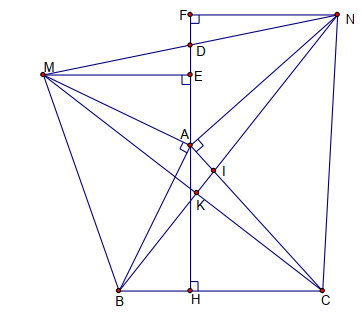
\includegraphics[width=0.45\textwidth]{14-4-lg.png}$$
    \begin{enumerate}
        \item Xét $\triangle \mathrm{AMC}$ và $\triangle \mathrm{ABN}$, có:\\[5pt]
        $\mathrm{AM}=\mathrm{AB}$ ( $\Delta \mathrm{AMB}$ vuông cân)\\[5pt]
        $\mathrm{AC}=\mathrm{AN}$ ( $\triangle \mathrm{ACN}$ vuông cân)\\[5pt]
        $\angle \mathrm{MAC}=\angle \mathrm{NAC}\left(=90^{\circ}+\angle \mathrm{BAC}\right)$\\[5pt]
        Suy ra $\Delta \mathrm{AMC}=\Delta \mathrm{ABN}(\mathrm{c}-\mathrm{g}-\mathrm{c})$
        \item Gọi I là giao điểm của $\mathrm{BN}$ với $\mathrm{AC}, \mathrm{K}$ là giao điểm của $\mathrm{BN}$ với $\mathrm{MC}$.\\[5pt]
        Xét $\Delta \mathrm{KIC}$ và $\Delta \mathrm{AIN}$, có:
        $\angle \mathrm{ANI}=\angle \mathrm{KCI}(\triangle \mathrm{AMC}=\Delta \mathrm{ABN}) \\[5pt]
        \angle \mathrm{AIN}=\angle \mathrm{KIC}$ (đối đỉnh)\\[5pt]
        $\Rightarrow \angle \mathrm{IKC}=\angle \mathrm{NAI}=90^{\circ} \text {, do đó: } \mathrm{MC} \perp \mathrm{BN}$
        \item Kẻ $\mathrm{ME} \perp \mathrm{AH}$ tại $\mathrm{E}, \mathrm{NF} \perp \mathrm{AH}$ tại $\mathrm{F}$. Gọi $\mathrm{D}$ là giao điểm của $\mathrm{MN}$ và $\mathrm{AH}$.\\[5pt]
        - Ta có: $\angle \mathrm{BAH}+\angle \mathrm{MAE}=90^{\circ}$ (vì $\angle \mathrm{MAB}=90^{\circ}$ )\\[5pt]
        Lại có $\angle \mathrm{MAE}+\angle \mathrm{AME}=90^{\circ}$, nên $\angle \mathrm{AME}=\angle \mathrm{BAH}$\\[5pt]
        Xét $\triangle \mathrm{MAE}$ và $\triangle \mathrm{ABH}$, vuông tại $\mathrm{E}$ và $\mathrm{H}$, có:\\[5pt]
        $\angle \mathrm{AME}=\angle \mathrm{BAH}$ (chứng minh trên)\\[5pt]
        $\mathrm{MA}=\mathrm{AB}$\\[5pt]
        Suy ra $\triangle \mathrm{MAE}=\triangle \mathrm{ABH}$ (cạnh huyền-góc nhọn)\\[5pt]
        $\Rightarrow \mathrm{ME}=\mathrm{AH}$\\[5pt]
        - Chứng minh tương tự ta có $\Delta_{\mathrm{AFN}}=\Delta_{\mathrm{CHA}}$\\[5pt]
        $\Rightarrow \mathrm{FN}=\mathrm{AH}$\\[5pt]
        Xét $\triangle \mathrm{MED}$ và $\triangle \mathrm{NFD}$, vuông tại $\mathrm{E}$ và $\mathrm{F}$, có:\\[5pt]
        $\mathrm{ME} =\mathrm{NF}(=\mathrm{AH}) \\[5pt]
        \angle \mathrm{EMD} =\angle \mathrm{FND}(\text { phụ với } \angle \mathrm{MDE} \text { và } \angle \mathrm{FDN} \text {, mà } \angle \mathrm{MDE}=\angle \mathrm{FDN}) \\[5pt]
        \Rightarrow \Delta \mathrm{MED} =\Delta \mathrm{NFD}\\[5pt] \Rightarrow \mathrm{BD}=\mathrm{ND} \text {. }$\\[5pt]
        Vậy $\mathrm{AH}$ đi qua trung điểm của $\mathrm{MN}$.
    \end{enumerate}
}
\end{bt}

\begin{bt}
    Cho ba số $\mathrm{a}, \mathrm{b}, \mathrm{c}$ thõa mãn: $0 \leq a \leq b+1 \leq c+2$ và $\mathrm{a}+\mathrm{b}+\mathrm{c}=1$. Tìm giá trị nhỏ nhất của c.
\loigiai{
        $\text {Vì: } 0 \leq a \leq b+1 \leq c+2 \text { nên } 0 \leq a+b+1+c+2 \leq c+2+c+2+c+2 \\
        \Rightarrow 0 \leq 4 \leq 3 c+6(\text { vì } \mathrm{a}+\mathrm{b}+\mathrm{c}=1) \\
        \text {Hay } 3 c \geq-2 \Rightarrow c \geq-\frac{2}{3}\\
        \text {Vậy giá trị nhỏ nhất của c là: }-\frac{2}{3} \text { khi đó } a+b=\frac{5}{3}$
}
\end{bt}